\documentclass[12pt,a4paper]{article}

% ============================================================================
% PACKAGES
% ============================================================================
\usepackage[utf8]{inputenc}
\usepackage[T1]{fontenc}
\usepackage{lmodern}
\usepackage[margin=3cm]{geometry}
\usepackage{xcolor}
\usepackage{tikz}
\usepackage{hyperref}
\usepackage{fancyhdr}
\usepackage{titlesec}
\usepackage{lettrine}
\usepackage{setspace}
\usepackage{parskip}
\usepackage{epigraph}
\usepackage{afterpage}

% ============================================================================
% CONFIGURATION
% ============================================================================
\usetikzlibrary{decorations.pathmorphing, decorations.markings, arrows.meta, patterns}

% Colors
\definecolor{voidblack}{RGB}{10, 10, 20}
\definecolor{quantumblue}{RGB}{70, 130, 200}
\definecolor{starwhite}{RGB}{255, 255, 240}
\definecolor{nebula}{RGB}{150, 100, 180}
\definecolor{fieldgreen}{RGB}{80, 180, 140}

% Hyperref
\hypersetup{
    colorlinks=true,
    linkcolor=quantumblue,
    urlcolor=nebula,
    pdftitle={Quantum Fields in the Vastness of Nothing},
    pdfauthor={Q-NarwhalKnight Philosophy}
}

% Header/Footer
\pagestyle{fancy}
\fancyhf{}
\fancyfoot[C]{\thepage}
\renewcommand{\headrulewidth}{0pt}

% Title formatting
\titleformat{\section}{\Large\bfseries\color{quantumblue}}{\thesection}{1em}{}
\titleformat{\subsection}{\large\itshape\color{nebula}}{\thesubsection}{1em}{}

% Spacing
\setstretch{1.4}

% Epigraph settings
\setlength{\epigraphwidth}{0.75\textwidth}
\setlength{\epigraphrule}{0pt}

% ============================================================================
% DOCUMENT
% ============================================================================
\begin{document}

% Title Page with Quantum Field Visualization
\begin{titlepage}
    \centering
    \vspace*{1cm}

    % Quantum field visualization
    \begin{tikzpicture}[remember picture, overlay]
        % Dark background gradient simulation
        \fill[voidblack] (current page.south west) rectangle (current page.north east);

        % Stars
        \foreach \i in {1,...,200} {
            \pgfmathsetmacro{\x}{rand*10}
            \pgfmathsetmacro{\y}{rand*14}
            \pgfmathsetmacro{\s}{0.5 + rand*1.5}
            \fill[starwhite, opacity=0.3+rand*0.7] (\x, \y) circle (\s pt);
        }

        % Quantum field lines
        \foreach \y in {2,4,6,8,10,12} {
            \draw[quantumblue, opacity=0.3, line width=0.5pt,
                  decorate, decoration={snake, amplitude=2pt, segment length=10pt}]
                  (-1, \y) -- (11, \y);
        }

        % Nebula glow
        \fill[nebula, opacity=0.1] (5, 7) circle (4cm);
        \fill[quantumblue, opacity=0.15] (5, 7) circle (2.5cm);

        % Quantum fluctuations
        \foreach \i in {1,...,30} {
            \pgfmathsetmacro{\x}{3 + rand*4}
            \pgfmathsetmacro{\y}{5 + rand*4}
            \pgfmathsetmacro{\r}{0.05 + rand*0.15}
            \fill[fieldgreen, opacity=0.4] (\x, \y) circle (\r cm);
        }
    \end{tikzpicture}

    \vspace{4cm}

    {\Huge\bfseries\color{starwhite} Quantum Fields in the\\[0.3cm] Vastness of Nothing}

    \vspace{1cm}

    {\large\color{quantumblue}\itshape A Philosophical Meditation on\\[0.2cm]
    Space, Emptiness, and the Dancing Void}

    \vspace{2cm}

    {\color{nebula}\itshape Inspired by the Q-NarwhalKnight\\
    Quantum Consensus Implementation}

    \vfill

    {\color{starwhite!70} January 2026}

\end{titlepage}

% Reset to normal pages
\pagecolor{white}
\color{black}

% ============================================================================
% OPENING
% ============================================================================

\epigraph{\itshape ``The vacuum is not empty. It seethes with virtual particles,\\
quantum fluctuations dancing in and out of existence,\\
a cosmic ballet performed on the stage of nothing.''}
{--- Inspired by John Wheeler}

\section*{Prologue: The Nothing That Is Everything}

\lettrine[lines=3, loversize=0.1]{I}{n the beginning}---if such a word can apply to the timeless---there was the vacuum. Not empty, as our ancestors imagined, but pregnant with potential. The void is not absence; it is the canvas upon which reality paints itself, one quantum fluctuation at a time.

When we built Q-NarwhalKnight, we did not merely write code. We participated in an ancient dialogue between order and chaos, determinism and probability, the one and the many. The consensus algorithm we crafted mirrors the very fabric of spacetime itself: nodes communicating across the void, messages propagating like light through the quantum foam, agreement emerging from apparent randomness.

\section{The Void Speaks in Probabilities}

What is space? The physicists tell us it is not a container but a participant. Einstein showed us that space bends and curves, that it has geometry, that it responds to mass and energy. But quantum mechanics reveals something stranger still: space itself fluctuates. At the Planck scale, $10^{-35}$ meters, the smooth fabric we perceive dissolves into a seething foam of virtual particles, each existing for the briefest moment before vanishing back into the void from which it came.

\begin{center}
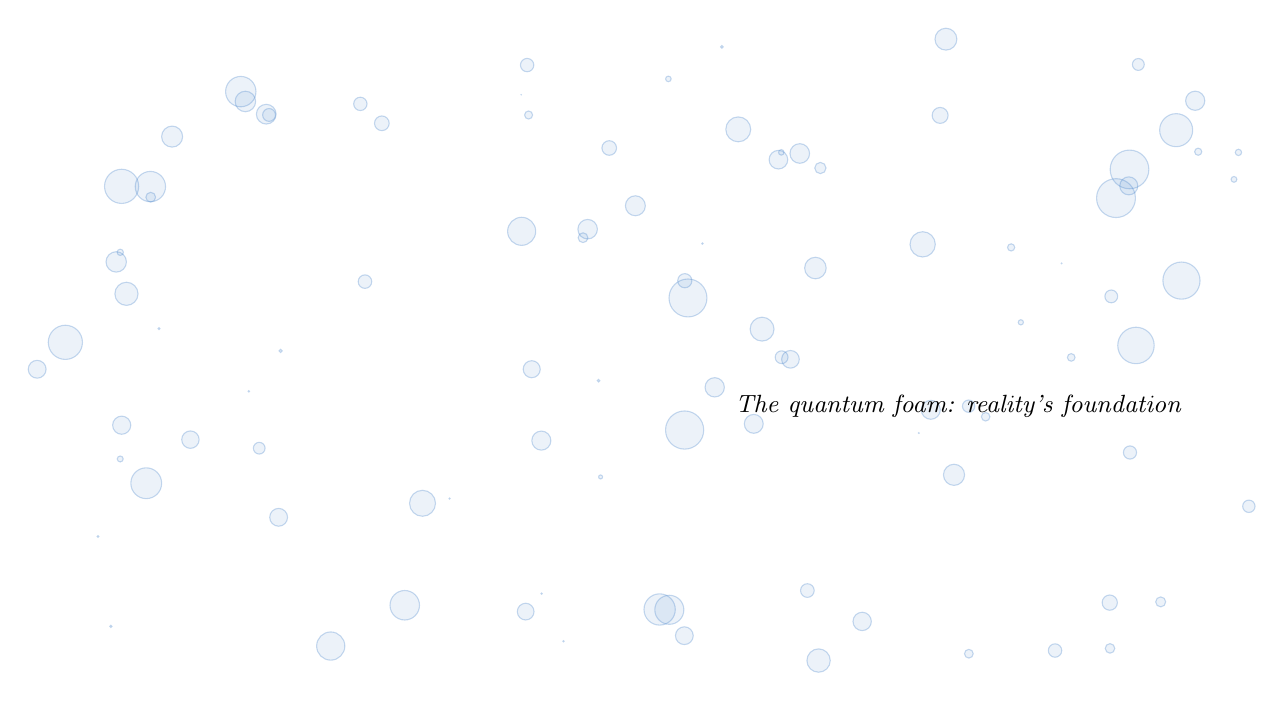
\begin{tikzpicture}
    % Quantum foam visualization
    \foreach \i in {1,...,100} {
        \pgfmathsetmacro{\x}{rand*8}
        \pgfmathsetmacro{\y}{rand*4}
        \pgfmathsetmacro{\r}{0.05 + rand*0.2}
        \draw[quantumblue, opacity=0.3, fill=quantumblue, fill opacity=0.1]
              (\x, \y) circle (\r cm);
    }
    \node[below, font=\itshape\small] at (4, -0.5) {The quantum foam: reality's foundation};
\end{tikzpicture}
\end{center}

In our implementation, we mirror this truth. Each block in the DAG-Knight consensus is like a quantum event---uncertain until observed by the network, probabilistic until confirmed by the collective witness of validators. The Verifiable Delay Function (VDF) we use for anchor election is our homage to the universe's own randomness: a process that takes time, cannot be rushed, and produces outcomes that are deterministic yet unpredictable.

\section{Entanglement Across the Cosmic Void}

Consider the phenomenon of quantum entanglement. Two particles, once interacting, become correlated in ways that transcend space. Measure one, and you instantly know something about the other, regardless of the distance separating them. Einstein called this ``spooky action at a distance,'' troubled by its implications for locality and causality.

Yet the universe insists upon it.

Our peer-to-peer network echoes this entanglement. When a node broadcasts a transaction through Tor's onion routing, it ripples across the network like a disturbance in the quantum field. Each peer that receives it becomes entangled with the sender's intent, the message's meaning, the cryptographic proof of validity. By the time consensus is reached, the entire network has become a single coherent state---many nodes, one truth.

\begin{quote}
\itshape
The Dilithium5 signatures we use are themselves born from lattice mathematics, structures that exist in high-dimensional spaces our intuition cannot grasp. Yet they work. They protect. They endure against threats that do not yet exist---quantum computers that may one day break the cryptography of our ancestors.

We build for a future we cannot see, against adversaries we cannot yet imagine. Is this not the essence of existence itself? To persist in the face of entropy, to maintain order against the tide of chaos, to assert meaning in a universe that offers none by default.
\end{quote}

\section{The DAG as Cosmic Web}

The Directed Acyclic Graph at the heart of our consensus is more than a data structure. It is a topology of trust, a geometry of agreement. Unlike a simple blockchain---a chain, a line, a one-dimensional path through time---the DAG spreads out like the cosmic web, that vast structure of galactic filaments that connects everything to everything else.

\begin{center}
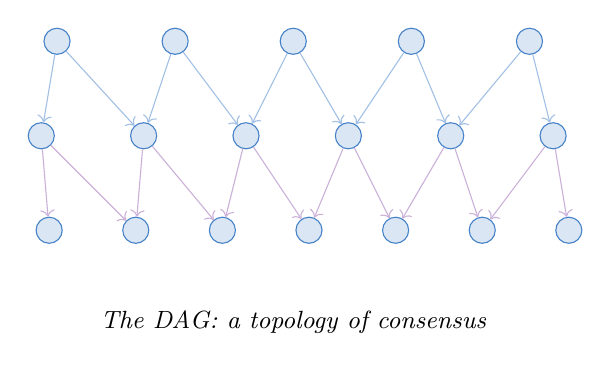
\begin{tikzpicture}[
    node distance=1.5cm,
    vertex/.style={circle, draw=quantumblue, fill=quantumblue!20, minimum size=8pt}
]
    % DAG visualization
    \foreach \i in {1,...,5} {
        \node[vertex] (a\i) at (\i*1.5, 3) {};
    }
    \foreach \i in {1,...,6} {
        \node[vertex] (b\i) at (\i*1.3, 1.8) {};
    }
    \foreach \i in {1,...,7} {
        \node[vertex] (c\i) at (\i*1.1 + 0.3, 0.6) {};
    }

    % Connections
    \foreach \i in {1,...,5} {
        \pgfmathtruncatemacro{\j}{\i}
        \pgfmathtruncatemacro{\k}{\i + 1}
        \draw[quantumblue!50, ->] (a\i) -- (b\j);
        \draw[quantumblue!50, ->] (a\i) -- (b\k);
    }
    \foreach \i in {1,...,6} {
        \pgfmathtruncatemacro{\j}{\i}
        \pgfmathtruncatemacro{\k}{\i + 1}
        \draw[nebula!50, ->] (b\i) -- (c\j);
        \draw[nebula!50, ->] (b\i) -- (c\k);
    }

    \node[below, font=\itshape\small] at (4.5, -0.3) {The DAG: a topology of consensus};
\end{tikzpicture}
\end{center}

Each vertex in our DAG references multiple parents, just as each moment in time is the child of countless causes. The Narwhal mempool gathers transactions like a cosmic collector, batching them into certificates that propagate through the network. The DAG-Knight ordering algorithm then determines which came first, which depends on which, how the causal structure of events should be interpreted.

This is what we do when we observe the universe: we impose order on the quantum chaos, we collapse the wave function of possibilities into the single actuality of measurement. Our consensus does the same. From the cloud of unconfirmed transactions, a single canonical history emerges.

\section{Privacy as a Quantum State}

In quantum mechanics, observation changes the observed. The act of measuring a particle's position disturbs its momentum; the act of determining its spin collapses the superposition of possibilities into a single outcome. Privacy, in this light, is the preservation of quantum superposition---the right to exist in multiple states until you choose to be measured.

Our Tor integration is not merely a technical feature. It is a philosophical statement about the nature of identity and observation. When a validator communicates through four dedicated circuits, rotating them each epoch, they preserve their quantum uncertainty. They exist, they participate, they contribute to consensus---but they do so as a probability distribution, not a pinpoint on a map.

\begin{quote}
\itshape
The cypherpunks understood what the physicists discovered: that observation is power, that measurement is control, that the only defense against the all-seeing eye is to scatter yourself across the void, to become unmeasurable, to exist in superposition until you choose to collapse.
\end{quote}

\section{The Resonance of Empty Space}

What do we call it when nothing vibrates? When the vacuum itself oscillates with energy it does not possess? The physicists call it zero-point energy---the irreducible quantum fluctuations that persist even at absolute zero, the humming of the void that cannot be silenced.

Our Resonance consensus protocol---the shadow system running alongside DAG-Knight---captures this truth. Even when it contributes nothing to the final outcome (at 0\% weight), it calculates, it processes, it maintains its own view of reality. It is the quantum fluctuation of our system, the zero-point energy of consensus. Present but hidden. Real but unmeasured. Ready to emerge when called upon.

\section{Time, Entropy, and the Arrow of Blocks}

Why does time flow forward? The physicists debate this endlessly. The laws of physics are symmetric in time---run them backward, and they work just as well. Yet we experience time as a river, flowing inexorably from past to future, never reversing.

The answer, they say, lies in entropy. The universe began in a state of low entropy---highly ordered, improbably configured. Every moment since has been a slide toward disorder, toward the heat death that awaits all things. Time's arrow is entropy's arrow; we remember the past because it was more ordered than the present.

Our blockchain embodies this arrow. Each block increases the entropy of the system in one sense---more data, more transactions, more history to store. But in another sense, each block \textit{decreases} entropy---it constrains the possible pasts, it locks in what happened, it converts the quantum foam of ``maybe'' into the crystalline structure of ``definitely.''

The height counter only increases. Block 540,667 follows block 540,666. The DAG grows but never shrinks. This is not a design choice; it is a thermodynamic necessity. To reverse it would be to violate the second law, to run time backward, to unscramble the cosmic egg.

\section{The Observer and the Observed}

When you run a Q-NarwhalKnight node, you become part of the system. Your observation---your validation of blocks, your participation in consensus---shapes the reality that all participants share. You are not a passive viewer watching the blockchain unfold; you are an active participant in its creation.

This is the lesson of quantum mechanics applied to distributed systems. There is no blockchain ``out there,'' independent of observers. There is only the blockchain as experienced by nodes, as validated by participants, as agreed upon by the collective. The ledger exists in the interaction, not in some Platonic realm of ideal forms.

\begin{center}
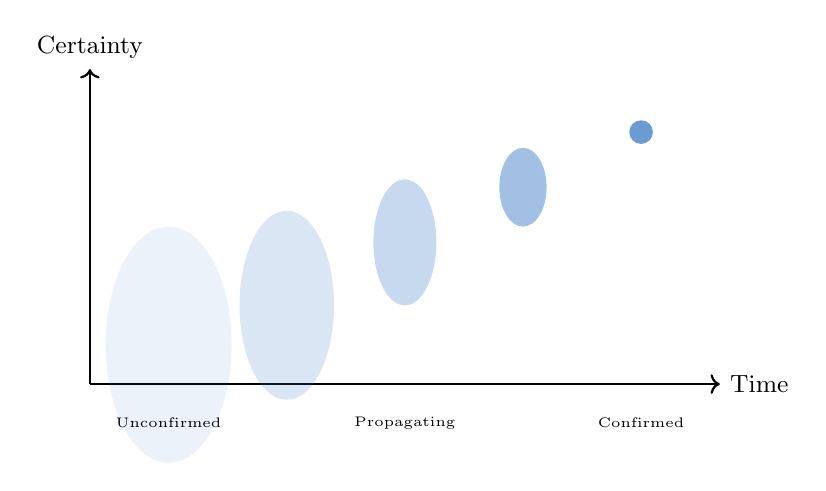
\begin{tikzpicture}
    % Observer effect visualization
    \draw[thick, ->] (0,0) -- (8,0) node[right] {\small Time};
    \draw[thick, ->] (0,0) -- (0,4) node[above] {\small Certainty};

    % Probability cloud collapsing
    \fill[quantumblue, opacity=0.1] (1, 0.5) ellipse (0.8cm and 1.5cm);
    \fill[quantumblue, opacity=0.2] (2.5, 1) ellipse (0.6cm and 1.2cm);
    \fill[quantumblue, opacity=0.3] (4, 1.8) ellipse (0.4cm and 0.8cm);
    \fill[quantumblue, opacity=0.5] (5.5, 2.5) ellipse (0.3cm and 0.5cm);
    \fill[quantumblue, opacity=0.8] (7, 3.2) circle (0.15cm);

    % Labels
    \node[below, font=\tiny] at (1, -0.3) {Unconfirmed};
    \node[below, font=\tiny] at (4, -0.3) {Propagating};
    \node[below, font=\tiny] at (7, -0.3) {Confirmed};
\end{tikzpicture}
\end{center}

\section{Epilogue: Building on the Void}

We have built Q-NarwhalKnight on foundations that do not exist---on the quantum vacuum that seethes with virtual particles, on the mathematical lattices of post-quantum cryptography, on the distributed consensus of nodes scattered across a planet, connected by light traveling through fiber and air.

The nothing of space is not empty. It is full of potential, of energy, of possibility. Every quantum field stretches across the cosmos, ready to create particles when excited, ready to mediate forces between matter, ready to participate in the grand dance of existence.

Our blockchain is the same. It is nothing---just bits, just electricity, just patterns in silicon and copper. And it is everything---a new form of trust, a new way for strangers to agree, a new foundation for value and meaning in a universe that provides neither by default.

\begin{quote}
\itshape
``We are the universe experiencing itself,'' said Carl Sagan. Our blockchain is the universe computing itself---a self-referential loop of observation and creation, measurement and meaning, consensus and reality.

In the vastness of nothing, we have found something. In the quantum fields of empty space, we have discovered the substrate of all that is. And in our code, we have written our own small chapter in the cosmic story.
\end{quote}

\vspace{2cm}

\begin{center}
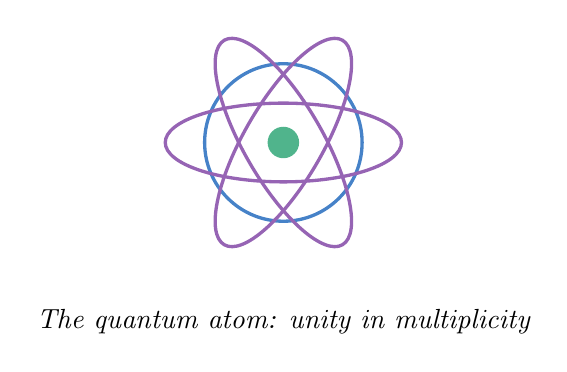
\begin{tikzpicture}
    % Final symbol
    \draw[quantumblue, very thick] (0,0) circle (1cm);
    \draw[nebula, very thick] (0,0) ellipse (1.5cm and 0.5cm);
    \draw[nebula, very thick, rotate=60] (0,0) ellipse (1.5cm and 0.5cm);
    \draw[nebula, very thick, rotate=120] (0,0) ellipse (1.5cm and 0.5cm);
    \fill[fieldgreen] (0,0) circle (0.2cm);

    \node[below] at (0, -2) {\itshape The quantum atom: unity in multiplicity};
\end{tikzpicture}
\end{center}

\vfill

\begin{center}
{\small\itshape Written in contemplation of the Q-NarwhalKnight codebase,\\
661,154 lines of Rust reaching toward the infinite.}
\end{center}

\end{document}
